\documentclass[tikz,border=2pt]{standalone}
\usepackage{amsmath,amssymb}
\usetikzlibrary{arrows.meta,decorations.pathreplacing}
\newcommand{\angl}[1]{\vbox{\hrule height0.4pt\hbox{$\scriptstyle #1\kern1pt$\vrule width0.4pt}}}
\begin{document}
% Annual annuity-due with a 5-year guarantee: payments at 0,...,4 are certain (annuity certain, PV 4.5);
% payments at 5,6,... are made only while the annuitant survives (5-year deferred life annuity, APV 8).
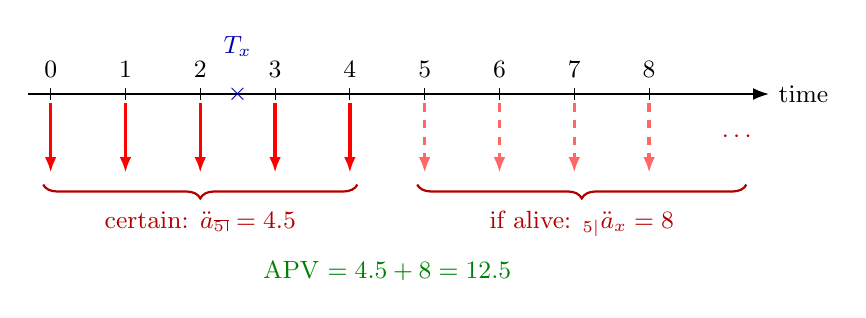
\begin{tikzpicture}[font=\small, >={Latex[length=2mm]}, x=0.95cm]
  \draw[->] (-0.3,0) -- (9.6,0) node[right] {time};
  \foreach \k in {0,...,8} {
    \draw (\k,0.08) -- (\k,-0.08);
    \node[anchor=south] at (\k,0.08) {$\k$};
  }
  % certain payments
  \foreach \k in {0,...,4} \draw[->, red, very thick] (\k,-0.12) -- (\k,-1.0);
  % life-contingent payments
  \foreach \k in {5,...,8} \draw[->, red!60, very thick, dashed] (\k,-0.12) -- (\k,-1.0);
  \node[red!70!black] at (9.2,-0.55) {$\cdots$};
  % early death
  \node[blue!70!black, font=\small\bfseries] at (2.5,0) {$\times$};
  \node[blue!70!black, anchor=south] at (2.5,0.35) {$T_x$};
  % braces
  \draw[red!70!black, thick, decorate, decoration={brace, mirror, amplitude=5pt}]
    (-0.1,-1.15) -- (4.1,-1.15) node[midway, below=6pt] {certain: $\ddot a_{\angl{5}}=4.5$};
  \draw[red!70!black, thick, decorate, decoration={brace, mirror, amplitude=5pt}]
    (4.9,-1.15) -- (9.3,-1.15) node[midway, below=6pt] {if alive: ${}_{5|}\ddot a_x=8$};
  \node[green!50!black] at (4.5,-2.25) {APV $=4.5+8=12.5$};
\end{tikzpicture}
\end{document}
